\chapter[Integrationsprozesse]{Integrationsprozesse}

Anschließend an die Beschreibung einer datengesteuerten Organisation, dessen Aufbau, Prozesse und Rollen werden innerhalb dieses Kapitels die Herausforderungen und Vorgehenswege zur Transformation in eine datengesteuerte Organisation thematisiert.

\section{Herausforderungen}

Bereits durch das sich äußere, sich schnell wechselnde kompetitive Umfeld einer Organisation, verkompliziert sich der Prozess datengesteuert z. B. Strategieentscheidungen in Organisation zu treffen. \footcite[Vgl.][S. 2]{Pratt.2023} 
Hinzu zu der Geschwindigkeit der Geschäftsumgebung, konnte durch eine Gartner Umfrage festgestellt werden, dass 65 \% der Teilnehmenden im Zeitraum der letzten zwei Jahre (2021-2023) einen Zuwachs in der Komplexität der Entscheidungen verzeichneten. \footcite[Vgl.][S. 65]{Pratt.2023}
Damit ist das Ableitungen von Strategieentscheidungen ein besonders herausforderndes Feld aufgrund der hoch diversen Daten und der Vielzahl von Einflussvariablen. \footcite[Vgl.][S. 3]{Pratt.2023}

Dieser äußere Einfluss wirkt sich dadurch ebenfalls erschwerend auf die internen managementbezogenen und kulturellen Herausforderungen aus, welche durch die Transformation zur datengesteuerten Organisation entstehen. \footcite[Vgl.][S. 15]{Dalpiaz.2020}
Bestätigt wird dies von \Citeauthor*{Dalpiaz.2020} durch die Forschungsergebnisse der Auswertung von 15 Interviews aus neun verschiedenen Software Unternehmen.
Aus den Interviews konnten die folgenden in Abbildung 4.1 dargelegte Herausforderungen in der Transformation zu einer datengesteuerten Organisation identifiziert werden. \footcite[][S. 9]{Dalpiaz.2020}

\begin{figure}[htb]
    \centering
    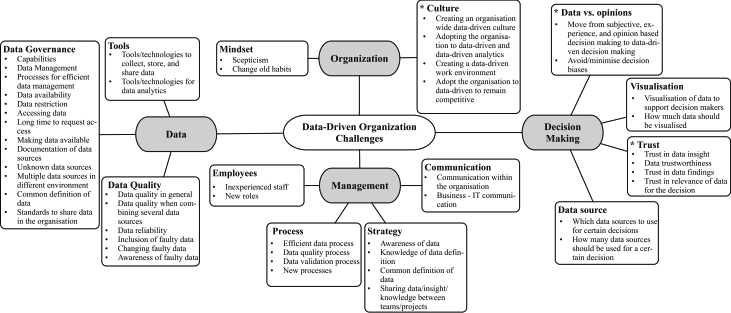
\includegraphics[width=0.95\textwidth]{graphics/DDO challenges.png}
    \caption{Herausforderungen einer datengesteuerten Organisation}
    \label{fig:DDOs challenges}
\end{figure}

Innerhalb der Grafik sind mittels \textbf{*} die drei wichtigsten Herausforderungen faktenbasierte Entscheidungen, Vertrauen und Kultur gekennzeichnet, welche alle 15 Teilnehmenden benannten.
Faktenbasierte Entscheidungen beschreibt die Absicht, subjektive, erfahrungsgestützte und meinungsbasierte Entscheidungen Mittels Daten durchzuführen oder bisherige Prozesse zu unterstützen. \footcite[Vgl.][S. 9]{Dalpiaz.2020}
Ein Einfluss auf die Umsetzung dieser Absicht nimmt die zweite Herausforderung des Vertrauens.
Für faktenbasierte Entscheidungen ist ein hohes Maß an Vertrauen gegenüber vielerlei Aspekte der Daten entlang des Data Science Prozesses notwendig.
Diese Aspekte umfassen die Aufnahme relevanter Daten, die fehlerfreie Aufnahme der Daten, die fehlerlose Verarbeitung der Daten sowie die korrekte Ableitung von für die Entscheidung relevanten Erkenntnissen. \footcite[Vgl.][S. 10]{Dalpiaz.2020}


\begin{itemize}
    \item outside view (fast and complex decisions)
    \item manageral and cultural challenges
    \item technical challenges
    \item need for DS framework
\end{itemize}

\section{Vorgehensmodelle zur Integration von Data Science}

\begin{itemize}
    \item Conceptual requirements
    \item Design Parameters
    \item Experiment Evolution Model (Microsoft)
    \item CSPG Framework
    \item DI / DS Integration Framework
\end{itemize}